\section{Question 3}
\subsection{Part a}
$x_1, x_2, x_3, x_4$ are all unconditionally independent of $x_6$. This is because the only possible path from $x_6$ to any of them uses $x_5$ as the center of a v-structure, and $x_5$ is not observed and has no observed descendants when no variables are observed, and hence cannot be the center of a v-structure. $x_5$ is dependent on $x_6$ because they are directly connected.  

\subsection{Part b}
$x_5$ is dependent on $x_6$. $x_4 \notindependent x_5 | S$ for any $S$ by virtue of a direct edge between them. $x_4 \notindependent x_6 | x_5$ by virtue of $x_5$ being a valid center of a v-structure.\\
$x_3 \notindependent x_5 | S$ and $x_3 \notindependent x_4 | S$ for any $S$.  $x_3 \notindependent x_6 | \{x_4, x_5\}$ due to $x_5$ being a valid center of a v-structure.\\
$x_2 \notindependent x_4 | S$ for any $S$. $x_2 \notindependent x_3 | x_4$. Thus, $x_2 \independent x_5, x_6 | \{x_4, x_3\}$ is the best we can do.\\
$x_1 \notindependent x_4 | S$ for any $S$. $x_1 \notindependent x_3 | x_4$ and $x_1 \notindependent x_2 | x_4$. Thus, $x_1 \independent x_5, x_6 | \{x_4, x_3, x_2\}$ is the best we can do.\\

\begin{figure}[H]
    \centering
    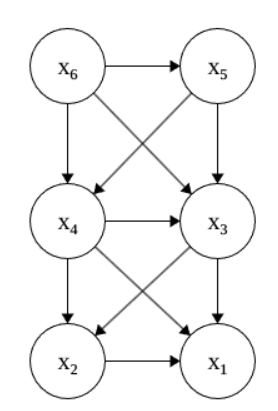
\includegraphics[width=0.3\textwidth]{../images/BN_Q3.png}
\end{figure}
